\documentclass[12pt]{beamer}\usepackage[]{graphicx}\usepackage[]{color}
%% maxwidth is the original width if it is less than linewidth
%% otherwise use linewidth (to make sure the graphics do not exceed the margin)
\makeatletter
\def\maxwidth{ %
  \ifdim\Gin@nat@width>\linewidth
    \linewidth
  \else
    \Gin@nat@width
  \fi
}
\makeatother

\definecolor{fgcolor}{rgb}{0.345, 0.345, 0.345}
\newcommand{\hlnum}[1]{\textcolor[rgb]{0.686,0.059,0.569}{#1}}%
\newcommand{\hlstr}[1]{\textcolor[rgb]{0.192,0.494,0.8}{#1}}%
\newcommand{\hlcom}[1]{\textcolor[rgb]{0.678,0.584,0.686}{\textit{#1}}}%
\newcommand{\hlopt}[1]{\textcolor[rgb]{0,0,0}{#1}}%
\newcommand{\hlstd}[1]{\textcolor[rgb]{0.345,0.345,0.345}{#1}}%
\newcommand{\hlkwa}[1]{\textcolor[rgb]{0.161,0.373,0.58}{\textbf{#1}}}%
\newcommand{\hlkwb}[1]{\textcolor[rgb]{0.69,0.353,0.396}{#1}}%
\newcommand{\hlkwc}[1]{\textcolor[rgb]{0.333,0.667,0.333}{#1}}%
\newcommand{\hlkwd}[1]{\textcolor[rgb]{0.737,0.353,0.396}{\textbf{#1}}}%
\let\hlipl\hlkwb

\usepackage{framed}
\makeatletter
\newenvironment{kframe}{%
 \def\at@end@of@kframe{}%
 \ifinner\ifhmode%
  \def\at@end@of@kframe{\end{minipage}}%
  \begin{minipage}{\columnwidth}%
 \fi\fi%
 \def\FrameCommand##1{\hskip\@totalleftmargin \hskip-\fboxsep
 \colorbox{shadecolor}{##1}\hskip-\fboxsep
     % There is no \\@totalrightmargin, so:
     \hskip-\linewidth \hskip-\@totalleftmargin \hskip\columnwidth}%
 \MakeFramed {\advance\hsize-\width
   \@totalleftmargin\z@ \linewidth\hsize
   \@setminipage}}%
 {\par\unskip\endMakeFramed%
 \at@end@of@kframe}
\makeatother

\definecolor{shadecolor}{rgb}{.97, .97, .97}
\definecolor{messagecolor}{rgb}{0, 0, 0}
\definecolor{warningcolor}{rgb}{1, 0, 1}
\definecolor{errorcolor}{rgb}{1, 0, 0}
\newenvironment{knitrout}{}{} % an empty environment to be redefined in TeX

\usepackage{alltt}
\usepackage{tikz}

% make it pretty
% get rid of junk
\usetheme{default}
\usefonttheme[onlymath]{serif}
\beamertemplatenavigationsymbolsempty

% define a bunch of colors
\definecolor{offwhite}{RGB}{255,250,240}
\definecolor{gray}{RGB}{155,155,155}
\definecolor{foreground}{RGB}{80,80,80}
\definecolor{background}{RGB}{255,255,255}
%\definecolor{title}{RGB}{255,199,0}
\definecolor{title}{RGB}{89,132,212}
%\definecolor{subtitle}{RGB}{89,132,212}
\definecolor{subtitle}{RGB}{255,199,0}
\definecolor{hilit}{RGB}{248,117,79}
\definecolor{vhilit}{RGB}{255,111,207}
\definecolor{lolit}{RGB}{200,200,200}
\definecolor{lit}{RGB}{255,199,0}
\definecolor{mdlit}{RGB}{89,132,212}
\definecolor{link}{RGB}{248,117,79}

% a few color macros
\newcommand{\hilit}{\color{hilit}}
\newcommand{\vhilit}{\color{vhilit}}
\newcommand{\lit}{\color{lit}}
\newcommand{\mdlit}{\color{mdlit}}
\newcommand{\lolit}{\color{lolit}}

% use those colors
\setbeamercolor{titlelike}{fg=title}
\setbeamercolor{subtitle}{fg=subtitle}
\setbeamercolor{frametitle}{fg=gray}
%\setbeamercolor{structure}{fg=subtitle}
\setbeamercolor{structure}{fg=title}
\setbeamercolor{institute}{fg=lolit}
\setbeamercolor{normal text}{fg=foreground,bg=background}
\setbeamertemplate{itemize subitem}{{\textendash}}
\setbeamerfont{itemize/enumerate subbody}{size=\small}
\setbeamerfont{itemize/enumerate subitem}{size=\small}

% center title of slides
\setbeamertemplate{blocks}[rounded]
\setbeamertemplate{frametitle}[default][center]

% page number
\setbeamerfont{page number in foot}{size=\footnotesize}
\setbeamertemplate{footline}[frame number]

% default link color
\hypersetup{colorlinks, urlcolor={link}}

% a few macros
\newcommand{\code}[1]{\texttt{#1}}
\newcommand{\hicode}[1]{{\hilit \texttt{#1}}}
\newcommand{\locode}[1]{{\lolit \texttt{#1}}}
\newcommand{\bb}[1]{\begin{block}{#1}}
\newcommand{\eb}{\end{block}}
\newcommand{\bi}{\begin{itemize}}
\newcommand{\bbi}{\vspace{4pt} \begin{itemize} \itemsep8pt}
\newcommand{\ei}{\end{itemize}}
\newcommand{\bv}{\begin{verbatim}}
\newcommand{\ev}{\end{verbatim}}
\newcommand{\ig}{\includegraphics}
\newcommand{\subt}[1]{{\footnotesize \color{subtitle} {#1}}}
\newcommand{\ttsm}{\tt \small}
\newcommand{\ttfn}{\tt \footnotesize}
\newcommand{\figh}[2]{\centerline{\includegraphics[height=#2\textheight]{#1}}}
\newcommand{\figw}[2]{\centerline{\includegraphics[width=#2\textwidth]{#1}}}



%------------------------------------------------

\title{Multicollinearity Issues in Linear Regression}
\subtitle{Intro 2 Statistical Learning}
\author{\href{http://www.gastonsanchez.com}{Gaston Sanchez}}
\institute{\href{https://creativecommons.org/licenses/by-sa/4.0/}{\tt \scriptsize \color{foreground} CC BY-SA 4.0}}
\date{}
\IfFileExists{upquote.sty}{\usepackage{upquote}}{}
\begin{document}



% no page number in first slide
{
  \setbeamertemplate{footline}{} 
  \frame{\titlepage} 
}

%------------------------------------------------

\begin{frame}
\frametitle{About}

Linear Regression Analysis (via OLS) relies on a series of assumptions 
that do not always hold. 

\bigskip
In these slides we focus on problems that arise from multicollinearity
in the predictors.

\bigskip
Also in these slides, I'm assuming that all variables (predictors and response)
are centered (mean = 0)!

\end{frame}

%------------------------------------------------

\begin{frame}
\frametitle{Main Assumptions in Linear Model}

The linear regression model of response $Y$ on predictors 
$X_1, X_2, \dots, X_p$ takes the form:

$$
Y = \beta_0 + \beta_1 X_1 + \beta_2 X_2 + \dots + \beta_p X_p + \varepsilon
$$

or in matrix notation: 

$$
\mathbf{y} = \mathbf{X} \boldsymbol{\beta} + \boldsymbol{\varepsilon}
$$

{\lit What are the main assumptions in this framework?}

\end{frame}

%------------------------------------------------

\begin{frame}
\frametitle{Main Assumptions in Linear Regression}

$$
\mathbf{y} = \mathbf{X} \boldsymbol{\beta} + \boldsymbol{\varepsilon}
$$

\bb{main assumptions}
\bi
  \item there is a linear relation between response and predictors
  \item the structural part of the model is $E(Y|X) = \mathbf{X} \boldsymbol{\beta}$
  \item $\boldsymbol{\varepsilon}$ is just ``noise'' (no systematic structure): \\
  $\boldsymbol{\varepsilon} \sim \text{i.i.d.} \hspace{2mm} N(\mathbf{0}, \sigma^2 \mathbf{I})$
  \item predictors are fairly linearly independent: \\
  $(\mathbf{X^\mathsf{T} X})$ is invertible
\ei
\eb

\end{frame}

%------------------------------------------------

\begin{frame}
\frametitle{Things that can fail}

\bbi
  \item Misspecified model (wrong structural part)
  \item Nonlinearity relation between response and predictors
  \item Dependence of errors
  \item Nonconstant variance of errors
  \item Lack of normality of errors
  \item {\hilit \textbf{Collinearity in Predictors}}
\ei

{\lolit We'll focus on collinearity in predictors}

\end{frame}

%------------------------------------------------

\begin{frame}
\begin{center}
\Huge{\hilit{Introduction}}
\end{center}
\end{frame}

%------------------------------------------------

\begin{frame}
\frametitle{Linear Regression}

Assuming centered data, the multiple regression model is:
$$
Y = \beta_1 X_1 + \beta_2 X_2 + \dots + \beta_p X_p + \varepsilon
$$

In matrix notation
{\Large
$$
\mathbf{y} = \mathbf{X} \boldsymbol{\beta} + \boldsymbol{\varepsilon}
$$
}

\end{frame}

%------------------------------------------------

\begin{frame}
\frametitle{Least Squares Solution}

The OLS solution is given by:
{\large
$$
\mathbf{\hat{y}} = \mathbf{X} \boldsymbol{\hat{\beta}} = \mathbf{X b}
$$
}

where:
{\large
$$
\mathbf{b} = \mathbf{(X^{\mathsf{T}} X)^{-1} X^{\mathsf{T}} y}
$$
}

\end{frame}

%------------------------------------------------

\begin{frame}
\begin{center}
\Huge{\hilit{Let's play with \code{mtcars}}}
\end{center}
\end{frame}

%------------------------------------------------

\begin{frame}[fragile]
\frametitle{Data set \code{mtcars}}

First 10 rows:
\begin{knitrout}\scriptsize
\definecolor{shadecolor}{rgb}{0.969, 0.969, 0.969}\color{fgcolor}\begin{kframe}
\begin{verbatim}
                   mpg cyl  disp  hp drat    wt  qsec vs am gear carb
Mazda RX4         21.0   6 160.0 110 3.90 2.620 16.46  0  1    4    4
Mazda RX4 Wag     21.0   6 160.0 110 3.90 2.875 17.02  0  1    4    4
Datsun 710        22.8   4 108.0  93 3.85 2.320 18.61  1  1    4    1
Hornet 4 Drive    21.4   6 258.0 110 3.08 3.215 19.44  1  0    3    1
Hornet Sportabout 18.7   8 360.0 175 3.15 3.440 17.02  0  0    3    2
Valiant           18.1   6 225.0 105 2.76 3.460 20.22  1  0    3    1
Duster 360        14.3   8 360.0 245 3.21 3.570 15.84  0  0    3    4
Merc 240D         24.4   4 146.7  62 3.69 3.190 20.00  1  0    4    2
Merc 230          22.8   4 140.8  95 3.92 3.150 22.90  1  0    4    2
Merc 280          19.2   6 167.6 123 3.92 3.440 18.30  1  0    4    4
\end{verbatim}
\end{kframe}
\end{knitrout}

Let's use \code{mpg} as response, and \code{disp}, \code{hp}, and \code{wt}
as predictors.

\end{frame}

%------------------------------------------------

\begin{frame}[fragile]
\frametitle{Data set \code{mtcars}}

\begin{knitrout}\footnotesize
\definecolor{shadecolor}{rgb}{0.969, 0.969, 0.969}\color{fgcolor}\begin{kframe}
\begin{alltt}
\hlcom{# response}
\hlstd{mpg} \hlkwb{<-} \hlstd{mtcars}\hlopt{$}\hlstd{mpg}

\hlcom{# predictors}
\hlstd{disp} \hlkwb{<-} \hlstd{mtcars}\hlopt{$}\hlstd{disp}
\hlstd{hp} \hlkwb{<-} \hlstd{mtcars}\hlopt{$}\hlstd{hp}
\hlstd{wt} \hlkwb{<-} \hlstd{mtcars}\hlopt{$}\hlstd{wt}

\hlcom{# standardized predictors}
\hlstd{X} \hlkwb{<-} \hlkwd{scale}\hlstd{(}\hlkwd{cbind}\hlstd{(disp, hp, wt))}
\end{alltt}
\end{kframe}
\end{knitrout}

\end{frame}

%------------------------------------------------

\begin{frame}[fragile]
\frametitle{Correlation matrix}

$$
\mathbf{R} = \frac{1}{n-1} \mathbf{X^\mathsf{T} X}
$$

\begin{knitrout}\footnotesize
\definecolor{shadecolor}{rgb}{0.969, 0.969, 0.969}\color{fgcolor}\begin{kframe}
\begin{alltt}
\hlcom{# correlation matrix}
\hlkwd{cor}\hlstd{(X)}
\end{alltt}
\begin{verbatim}
##           disp        hp        wt
## disp 1.0000000 0.7909486 0.8879799
## hp   0.7909486 1.0000000 0.6587479
## wt   0.8879799 0.6587479 1.0000000
\end{verbatim}
\end{kframe}
\end{knitrout}

\end{frame}

%------------------------------------------------

\begin{frame}[fragile]

\begin{knitrout}\footnotesize
\definecolor{shadecolor}{rgb}{0.969, 0.969, 0.969}\color{fgcolor}

{\centering 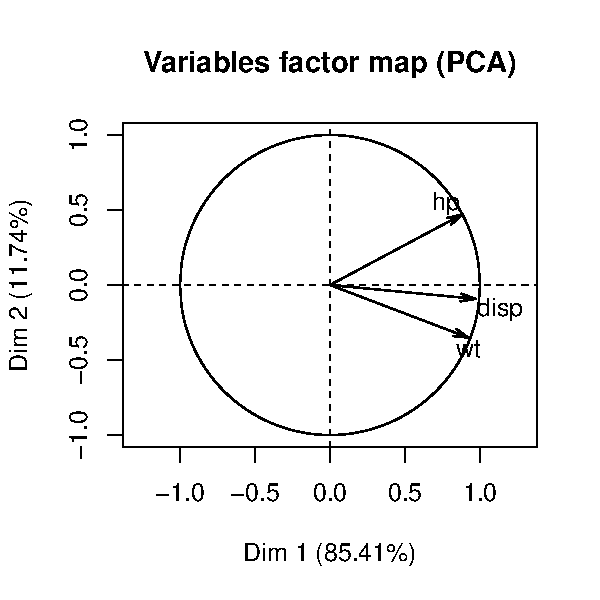
\includegraphics[width=.8\linewidth,height=.8\linewidth]{figure/pca-1} 

}



\end{knitrout}

\end{frame}

%------------------------------------------------

\begin{frame}[fragile]
\frametitle{LS Regression}

\begin{knitrout}\footnotesize
\definecolor{shadecolor}{rgb}{0.969, 0.969, 0.969}\color{fgcolor}\begin{kframe}
\begin{alltt}
\hlcom{# LS regression}
\hlstd{reg} \hlkwb{<-} \hlkwd{lm}\hlstd{(mpg} \hlopt{~} \hlstd{disp} \hlopt{+} \hlstd{hp} \hlopt{+} \hlstd{wt)}
\hlstd{reg}
\end{alltt}
\begin{verbatim}
## 
## Call:
## lm(formula = mpg ~ disp + hp + wt)
## 
## Coefficients:
## (Intercept)         disp           hp           wt  
##   37.105505    -0.000937    -0.031157    -3.800891
\end{verbatim}
\begin{alltt}
\hlcom{# regression summary}
\hlstd{reg_sum} \hlkwb{<-} \hlkwd{summary}\hlstd{(reg)}
\end{alltt}
\end{kframe}
\end{knitrout}

\end{frame}

%------------------------------------------------

\begin{frame}[fragile]
\frametitle{LS Regression}

\begin{knitrout}\scriptsize
\definecolor{shadecolor}{rgb}{0.969, 0.969, 0.969}\color{fgcolor}\begin{kframe}
\begin{verbatim}

Call:
lm(formula = mpg ~ disp + hp + wt)

Residuals:
   Min     1Q Median     3Q    Max 
-3.891 -1.640 -0.172  1.061  5.861 

Coefficients:
             Estimate Std. Error t value Pr(>|t|)    
(Intercept) 37.105505   2.110815  17.579  < 2e-16 ***
disp        -0.000937   0.010350  -0.091  0.92851    
hp          -0.031157   0.011436  -2.724  0.01097 *  
wt          -3.800891   1.066191  -3.565  0.00133 ** 
---
Signif. codes:  0 '***' 0.001 '**' 0.01 '*' 0.05 '.' 0.1 ' ' 1

Residual standard error: 2.639 on 28 degrees of freedom
Multiple R-squared:  0.8268,	Adjusted R-squared:  0.8083 
F-statistic: 44.57 on 3 and 28 DF,  p-value: 8.65e-11
\end{verbatim}
\end{kframe}
\end{knitrout}

\end{frame}

%------------------------------------------------

\begin{frame}[fragile]
\frametitle{LS Regression}

Ratio between std errors and coeffs
\begin{knitrout}\footnotesize
\definecolor{shadecolor}{rgb}{0.969, 0.969, 0.969}\color{fgcolor}\begin{kframe}
\begin{alltt}
\hlkwd{round}\hlstd{(reg_sum}\hlopt{$}\hlstd{coefficients[,}\hlnum{2}\hlstd{]} \hlopt{/} \hlstd{reg_sum}\hlopt{$}\hlstd{coefficients[,}\hlnum{1}\hlstd{],} \hlnum{4}\hlstd{)}
\end{alltt}
\begin{verbatim}
(Intercept)        disp          hp          wt 
     0.0569    -11.0455     -0.3670     -0.2805 
\end{verbatim}
\end{kframe}
\end{knitrout}

\code{disp} has a large standard error compared to its estimate

\end{frame}

%------------------------------------------------

\begin{frame}[fragile]
\frametitle{Inverse of $\mathbf{(X^\mathsf{T} X)}$}

What about $\mathbf{(X^\mathsf{T} X)^{-1}}$

\begin{knitrout}\footnotesize
\definecolor{shadecolor}{rgb}{0.969, 0.969, 0.969}\color{fgcolor}\begin{kframe}
\begin{alltt}
\hlkwd{solve}\hlstd{(}\hlkwd{t}\hlstd{(X)} \hlopt \hlstd{X)}
\end{alltt}
\begin{verbatim}
##             disp          hp          wt
## disp  0.23627475 -0.08598357 -0.15316573
## hp   -0.08598357  0.08827847  0.01819843
## wt   -0.15316573  0.01819843  0.15627798
\end{verbatim}
\end{kframe}
\end{knitrout}

\end{frame}

%------------------------------------------------

\begin{frame}
\begin{center}
\Huge{\hilit{Multicollinearity Issues}}
\end{center}
\end{frame}

%------------------------------------------------

\begin{frame}
\frametitle{Multicollinearity}

One of the issues when fitting regression models is due to multicollinearity:
the condition that arises when two or more predictors are highly correlated.

\bigskip
{\lit How does this affect OLS regression?}

\end{frame}

%------------------------------------------------

\begin{frame}
\frametitle{Exact Collinearity}

When one or more predictors are linear combinations of other predictors, then 
$\mathbf{X^\mathsf{T} X}$ is singular.

\bigskip
This is known as \textit{exact collinearity}.

\bigskip
There is no unique LS estimate $\hat{\boldsymbol{\beta}}$

\end{frame}

%------------------------------------------------

\begin{frame}
\frametitle{Multicollinearity: Near-exact Collinearity}

A more challenging problem arises when $\mathbf{X^\mathsf{T} X}$ is close to singular 
but not exactly.

\bigskip
This is usually referred to as \textit{multicollinearity}

\bigskip
Multicollinearity leads to imprecise (unstable) estimates $\boldsymbol{\hat{\beta}}$

\end{frame}

%------------------------------------------------

\begin{frame}
\frametitle{What causes multicollinearity?}

\bbi
  \item One or more predictors are linear combinations of other predictors
  \item One or more predictors are almost perfect linear combinations of other predictors
  \item More predictors than observations $p > n$
\ei

\end{frame}

%------------------------------------------------

\begin{frame}[fragile]
\frametitle{Exact Collinearity}

Let's introduce exact collinearity

\begin{knitrout}\footnotesize
\definecolor{shadecolor}{rgb}{0.969, 0.969, 0.969}\color{fgcolor}\begin{kframe}
\begin{alltt}
\hlstd{disp1} \hlkwb{<-} \hlnum{10} \hlopt{*} \hlstd{disp}

\hlstd{X1} \hlkwb{<-} \hlkwd{scale}\hlstd{(}\hlkwd{cbind}\hlstd{(disp, disp1, hp, wt))}

\hlkwd{solve}\hlstd{(}\hlkwd{t}\hlstd{(X1)} \hlopt \hlstd{X1)}
\end{alltt}


{\ttfamily\noindent\bfseries\color{errorcolor}{Error in solve.default(t(X1) \%*\% X1): system is computationally singular: reciprocal condition number = 1.55757e-17}}\end{kframe}
\end{knitrout}

{\lit Ooops!}

\end{frame}

%------------------------------------------------

\begin{frame}[fragile]

\begin{knitrout}\footnotesize
\definecolor{shadecolor}{rgb}{0.969, 0.969, 0.969}\color{fgcolor}

{\centering 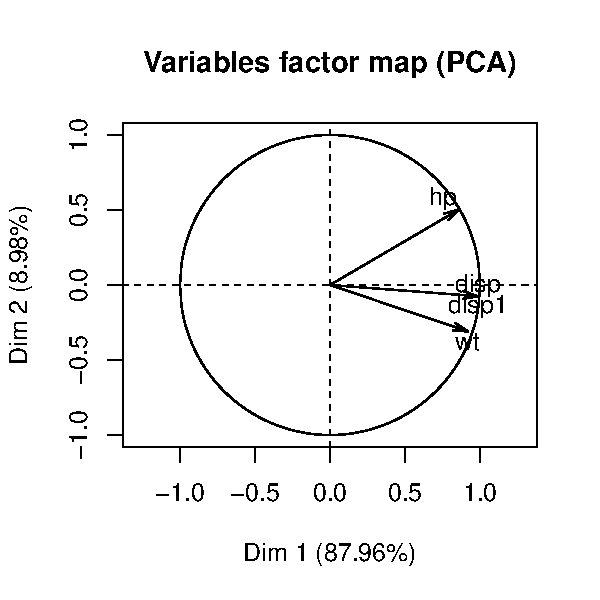
\includegraphics[width=.8\linewidth,height=.8\linewidth]{figure/pca1-1} 

}



\end{knitrout}

\end{frame}

%------------------------------------------------

\begin{frame}[fragile]
\frametitle{Near-exact Collinearity}

Let's introduce near-exact collinearity

\begin{knitrout}\footnotesize
\definecolor{shadecolor}{rgb}{0.969, 0.969, 0.969}\color{fgcolor}\begin{kframe}
\begin{alltt}
\hlkwd{set.seed}\hlstd{(}\hlnum{123}\hlstd{)}
\hlstd{disp2} \hlkwb{<-} \hlstd{disp} \hlopt{+} \hlkwd{rnorm}\hlstd{(}\hlkwd{length}\hlstd{(disp))}

\hlstd{X2} \hlkwb{<-} \hlkwd{scale}\hlstd{(}\hlkwd{cbind}\hlstd{(disp, disp2, hp, wt))}

\hlkwd{solve}\hlstd{(}\hlkwd{t}\hlstd{(X2)} \hlopt \hlstd{X2)}
\end{alltt}
\begin{verbatim}
             disp       disp2          hp          wt
disp   588.167214 -590.721826  1.01055902  1.99383316
disp2 -590.721826  593.525960 -1.10174784 -2.15719062
hp       1.010559   -1.101748  0.09032362  0.02220277
wt       1.993833   -2.157191  0.02220277  0.16411837
\end{verbatim}
\end{kframe}
\end{knitrout}

\end{frame}

%------------------------------------------------

\begin{frame}[fragile]

\begin{knitrout}\footnotesize
\definecolor{shadecolor}{rgb}{0.969, 0.969, 0.969}\color{fgcolor}

{\centering 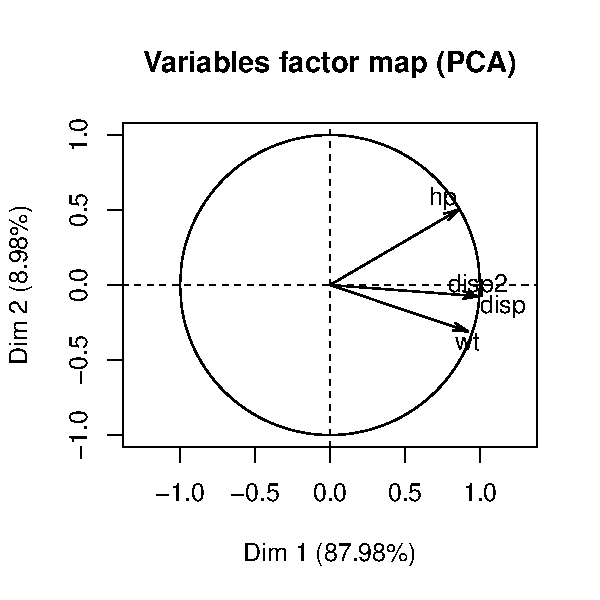
\includegraphics[width=.8\linewidth,height=.8\linewidth]{figure/pca2-1} 

}



\end{knitrout}

\end{frame}

%------------------------------------------------

\begin{frame}[fragile]
\frametitle{Near-exact Collinearity}

What about $X_j$ and $X_{j}^{2}$?

\begin{knitrout}\footnotesize
\definecolor{shadecolor}{rgb}{0.969, 0.969, 0.969}\color{fgcolor}\begin{kframe}
\begin{alltt}
\hlstd{disp_sqr} \hlkwb{<-} \hlstd{disp}\hlopt{^}\hlnum{2}

\hlstd{Xsqr} \hlkwb{<-} \hlkwd{scale}\hlstd{(}\hlkwd{cbind}\hlstd{(disp, disp_sqr, hp, wt))}

\hlkwd{solve}\hlstd{(}\hlkwd{t}\hlstd{(Xsqr)} \hlopt \hlstd{Xsqr)}
\end{alltt}
\begin{verbatim}
               disp    disp_sqr          hp          wt
disp      1.2157359 -0.91716163 -0.17616042 -0.16445287
disp_sqr -0.9171616  0.85882476  0.08444107  0.01056920
hp       -0.1761604  0.08444107  0.09658086  0.01923761
wt       -0.1644529  0.01056920  0.01923761  0.15640806
\end{verbatim}
\end{kframe}
\end{knitrout}

\end{frame}

%------------------------------------------------

\begin{frame}[fragile]

\begin{knitrout}\footnotesize
\definecolor{shadecolor}{rgb}{0.969, 0.969, 0.969}\color{fgcolor}

{\centering 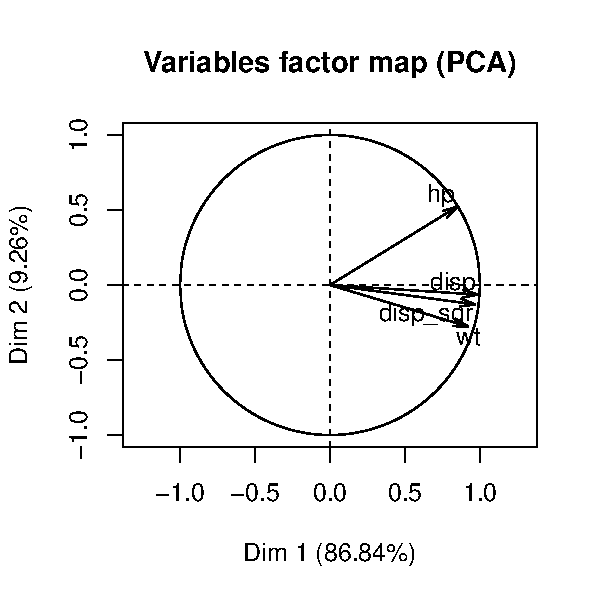
\includegraphics[width=.8\linewidth,height=.8\linewidth]{figure/pca3-1} 

}



\end{knitrout}

\end{frame}

%------------------------------------------------

\begin{frame}[fragile]
\frametitle{Multicollinearity}

Let's examine correlations of \code{disp} and cousins

\begin{knitrout}\footnotesize
\definecolor{shadecolor}{rgb}{0.969, 0.969, 0.969}\color{fgcolor}\begin{kframe}
\begin{alltt}
\hlkwd{cor}\hlstd{(}\hlkwd{cbind}\hlstd{(disp, disp_sqr, hp, wt))}
\end{alltt}
\begin{verbatim}
              disp  disp_sqr        hp        wt
disp     1.0000000 0.9792310 0.7909486 0.8879799
disp_sqr 0.9792310 1.0000000 0.7382463 0.8712214
hp       0.7909486 0.7382463 1.0000000 0.6587479
wt       0.8879799 0.8712214 0.6587479 1.0000000
\end{verbatim}
\end{kframe}
\end{knitrout}

\end{frame}

%------------------------------------------------

\begin{frame}[fragile]
\frametitle{Multicollinearity Issues}

\begin{knitrout}\footnotesize
\definecolor{shadecolor}{rgb}{0.969, 0.969, 0.969}\color{fgcolor}\begin{kframe}
\begin{alltt}
\hlkwd{solve}\hlstd{(}\hlkwd{t}\hlstd{(X2)} \hlopt \hlstd{X2)}
\end{alltt}
\begin{verbatim}
             disp       disp2          hp          wt
disp   588.167214 -590.721826  1.01055902  1.99383316
disp2 -590.721826  593.525960 -1.10174784 -2.15719062
hp       1.010559   -1.101748  0.09032362  0.02220277
wt       1.993833   -2.157191  0.02220277  0.16411837
\end{verbatim}
\begin{alltt}
\hlkwd{solve}\hlstd{(}\hlkwd{t}\hlstd{(Xsqr)} \hlopt \hlstd{Xsqr)}
\end{alltt}
\begin{verbatim}
               disp    disp_sqr          hp          wt
disp      1.2157359 -0.91716163 -0.17616042 -0.16445287
disp_sqr -0.9171616  0.85882476  0.08444107  0.01056920
hp       -0.1761604  0.08444107  0.09658086  0.01923761
wt       -0.1644529  0.01056920  0.01923761  0.15640806
\end{verbatim}
\end{kframe}
\end{knitrout}

\end{frame}

%------------------------------------------------

\begin{frame}
\begin{center}
\Huge{\mdlit{Let's make it \\ more extreme!}}
\end{center}
\end{frame}

%------------------------------------------------

\begin{frame}[fragile]
\frametitle{Extreme Multicollinearity}

\begin{knitrout}\footnotesize
\definecolor{shadecolor}{rgb}{0.969, 0.969, 0.969}\color{fgcolor}\begin{kframe}
\begin{alltt}
\hlkwd{set.seed}\hlstd{(}\hlnum{123}\hlstd{)}
\hlstd{disp3} \hlkwb{<-} \hlstd{disp} \hlopt{+} \hlkwd{rnorm}\hlstd{(}\hlkwd{length}\hlstd{(disp),} \hlkwc{mean} \hlstd{=} \hlnum{0}\hlstd{,} \hlkwc{sd} \hlstd{=} \hlnum{0.1}\hlstd{)}

\hlstd{X3} \hlkwb{<-} \hlkwd{scale}\hlstd{(}\hlkwd{cbind}\hlstd{(disp, disp3, hp, wt))}

\hlkwd{cor}\hlstd{(disp, disp3)}
\end{alltt}
\begin{verbatim}
[1] 0.9999997
\end{verbatim}
\end{kframe}
\end{knitrout}

\end{frame}

%------------------------------------------------

\begin{frame}[fragile]
\frametitle{Multicollinearity Issues}

\begin{knitrout}\footnotesize
\definecolor{shadecolor}{rgb}{0.969, 0.969, 0.969}\color{fgcolor}\begin{kframe}
\begin{alltt}
\hlcom{# small changes may have a "butterfly" effect}
\hlstd{disp31} \hlkwb{<-} \hlstd{disp3}

\hlcom{# change just one observation}
\hlstd{disp31[}\hlnum{1}\hlstd{]} \hlkwb{<-} \hlstd{disp3[}\hlnum{1}\hlstd{]} \hlopt{*} \hlnum{1.01}

\hlstd{X31} \hlkwb{<-} \hlkwd{scale}\hlstd{(}\hlkwd{cbind}\hlstd{(disp, disp31, hp, wt))}

\hlkwd{cor}\hlstd{(disp, disp31)}
\end{alltt}
\begin{verbatim}
[1] 0.9999973
\end{verbatim}
\end{kframe}
\end{knitrout}

\end{frame}

%------------------------------------------------

\begin{frame}[fragile]
\frametitle{Multicollinearity Issues}

\begin{knitrout}\footnotesize
\definecolor{shadecolor}{rgb}{0.969, 0.969, 0.969}\color{fgcolor}\begin{kframe}
\begin{alltt}
\hlkwd{solve}\hlstd{(}\hlkwd{t}\hlstd{(X3)} \hlopt \hlstd{X3)}
\end{alltt}
\begin{verbatim}
              disp        disp3           hp           wt
disp   59175.36325 -59202.97211  10.91501090  21.38646548
disp3 -59202.97211  59230.83035 -11.00617104 -21.54976679
hp        10.91501    -11.00617   0.09032362   0.02220277
wt        21.38647    -21.54977   0.02220277   0.16411837
\end{verbatim}
\begin{alltt}
\hlkwd{solve}\hlstd{(}\hlkwd{t}\hlstd{(X31)} \hlopt \hlstd{X31)}
\end{alltt}
\begin{verbatim}
                disp        disp31          hp          wt
disp    5941.5946101 -5942.3977358  0.30661752  0.64947961
disp31 -5942.3977358  5943.4373181 -0.39266978 -0.80278577
hp         0.3066175    -0.3926698  0.08830442  0.01825147
wt         0.6494796    -0.8027858  0.01825147  0.15638642
\end{verbatim}
\end{kframe}
\end{knitrout}

\end{frame}

%------------------------------------------------

\begin{frame}
\begin{center}
\Huge{\hilit{Variance of Coefficients \\ and Multicollinearity}}
\end{center}
\end{frame}

%------------------------------------------------

\begin{frame}
\frametitle{Variance-Covariance matrix $Var(\mathbf{\boldsymbol{\hat{\beta}}})$}

$$
Var(\mathbf{\boldsymbol{\hat{\beta}}}) = 
\
\begin{bmatrix} 
Var(\hat{\beta}_1) & Cov(\hat{\beta}_1, \hat{\beta}_2) & \cdots & Cov(\hat{\beta}_1, \hat{\beta}_p) \\
Cov(\hat{\beta}_2, \hat{\beta}_1) & Var(\hat{\beta}_2) & \cdots & Cov(\hat{\beta}_2, \hat{\beta}_p) \\
\vdots &  & \ddots & \vdots \\
Cov(\hat{\beta}_p, \hat{\beta}_1) & Cov(\hat{\beta}_p, \hat{\beta}_2) & \cdots & Var(\hat{\beta}_p) \\
\end{bmatrix}
$$

$$
Var(\mathbf{\boldsymbol{\hat{\beta}}}) = \sigma^2 (\mathbf{X^\mathsf{T} X})^{-1}
$$

\end{frame}

%------------------------------------------------

\begin{frame}
\frametitle{Variance of Estimates}

The variance-Covariance matrix $Var(\mathbf{\boldsymbol{\hat{\beta}}})$ is:
$$
Var(\boldsymbol{\hat{\beta}}) = \sigma^2 (\mathbf{X^\mathsf{T} X})^{-1}
$$

\bigskip
The variance of a particular coefficient $\hat{\beta}_j$ is given by:
$$
Var(\hat{\beta}_j) = \sigma^2 \left [ (\mathbf{X^\mathsf{T} X})^{-1} \right ]_{jj} 
$$

where $\left [ (\mathbf{X^\mathsf{T} X})^{-1} \right ]_{jj}$ is the $j$-th diagonal element
of $(\mathbf{X^\mathsf{T} X})^{-1}$

\end{frame}

%------------------------------------------------

\begin{frame}
\frametitle{Variance of Estimates}

\bbi
  \item Recall again that we don't know $\sigma^2$. How can we find an estimator 
  $\hat{\sigma}^2$?
  \item We don't observe the error terms $\boldsymbol{\varepsilon}$ but we do have
  the residuals $\mathbf{e = y - \hat{y}}$
  \item As well as the Residual Sum of Squares (RSS)
  $$
  \text{RSS} = \sum_{i=1}^{n} e_{i}^{2} = \sum_{i=1}^{n} (y_i - \hat{y}_i)^2
  $$
\ei

\end{frame}

%------------------------------------------------

\begin{frame}
\frametitle{Unbiased Estimate of $\sigma^2$}

To estimate $\sigma^2$ we use:
$$
\hat{\sigma}^2 = \frac{\text{RSS}}{n-p-1} = \frac{\sum_{i=1}^{n} (y_i - \hat{y}_i)^2}{n-p-1} = s^2
$$

The square root $\hat{\sigma} = \sqrt{\frac{\text{RSS}}{n-p-1}}$ is also known as the \\
\textbf{Residual Standard Error} {\lolit (reported by most software)}

\end{frame}

%------------------------------------------------

\begin{frame}
\frametitle{Variance Inflation Factor (VIF)}

Assuming standardized variables, $\mathbf{X^\mathsf{T} X} = n \mathbf{R}$

It can be shown that 
$$
Var(\boldsymbol{\hat{\beta}}) = \sigma^2 \left ( \frac{\mathbf{R}^{-1}}{n} \right )
$$

and $Var(\hat{\beta}_j)$ can then be expressed as:
$$
Var(\hat{\beta}_j) = \frac{\sigma^2}{n} [\mathbf{R}^{-1}]_{jj}
$$

\end{frame}

%------------------------------------------------

\begin{frame}
\frametitle{Variance Inflation Factor (VIF)}

$$
Var(\hat{\beta}_j) = \frac{\sigma^2}{n} [\mathbf{R}^{-1}]_{jj}
$$

It turns out that:
$$
[\mathbf{R}^{-1}]_{jj} = \frac{1}{1 - R_{j}^{2}}
$$
is known as the \textbf{Variance Inflation Factor} or VIF

\bigskip
If $R_{j}^{2}$ is close to 1, then VIF will be large, and so $Var(\hat{\beta})$ will also be large.

\end{frame}

%------------------------------------------------

\begin{frame}
\frametitle{Role of eigenvalues of matrix $\mathbf{R}$}

If we write the eigenvalue decomposition of $\mathbf{R}$ as:
{\large
$$
\mathbf{R = V \boldsymbol{\Lambda} V^\mathsf{T}}
$$
}

\pause
then the inverse of $\mathbf{R}$ becomes:
{\large
$$
\mathbf{R^{-1} = V \boldsymbol{\Lambda}^{-1} V^\mathsf{T}}
$$
}

\end{frame}

%------------------------------------------------

\begin{frame}
\frametitle{Role of eigenvalues of matrix $\mathbf{R}$}

It can be shown that 
$$
Var(\hat{\beta}_j) = \left ( \frac{\sigma^2}{n} \right )  \sum_{l=1}^{p} \frac{v^{2}_{jl}}{\lambda_l}
$$

As you can tell, the variance of the estimators depends on the inverses of the
eigenvalues of $\mathbf{R}$

\bigskip
With very small eigenvalues, the larger the variance of the estimates.

\end{frame}

%------------------------------------------------

\begin{frame}
\frametitle{In Summary}

\bb{With multicollinearity ...}
\bbi
  \item the standard errors of $\hat{\beta}_j$ are inflated.
  \item the fit is unstable, and becomes very sensitive to small perturbations.
  \item small changes in $Y$ can lead to large changes in the coefficients.
\ei
\eb

\end{frame}

%------------------------------------------------

\begin{frame}
\begin{center}
\Huge{\hilit{How to detect \\ Multicollinearity?}}
\end{center}
\end{frame}

%------------------------------------------------

\begin{frame}
\frametitle{How to detect Collinearity?}

\bbi
  \item Examine correlation matrix of predictors
  \item Check \textit{multiple correlation} coefficients $R_{j}^{2}$ \\
  {\small {\lolit $R_{j}^{2}$ is the coeff of determination when regressing $X_j$ on all other predictors}}
  \item Examine eigenvalues of $\mathbf{X^\mathsf{T} X}$
\ei

\end{frame}

%------------------------------------------------

\begin{frame}
\frametitle{Detecting collinearity pairwise correlations}

Perhaps the most basic approach to start checking whether there is multicollinearity
is to examine the (population) correlation matrix of predictors

{\Large
$$
\mathbf{R} = \frac{1}{n} \mathbf{X^\mathsf{T} X}
$$
}

\end{frame}

%------------------------------------------------

\begin{frame}
\frametitle{Detecting collinearity pairwise correlations}

\bb{Examining the correlation matrix}
\bbi
  \item Examining the correlation matrix of predictors
  \item Correlation values close to $-1$ or $+1$ indicate large 
  \textbf{pairwise} collinearities.
  \item However, there may be small correlations from highly correlated variables.
\ei
\eb

\end{frame}

%------------------------------------------------

\begin{frame}
\frametitle{Detecting collinearity with $R_{j}^{2}$ coefficients}

\bb{Multiple correlation coefficients}
\bbi
  \item Another way to check for collinearity is to calculate multiple correlation 
  coefficients $R_{j}^{2}$ for each predictor.
  \item Regress $X_j$ on all other predictors $X_h$ ($h \neq j$).
  \item If $R_{j}^{2}$ is close to one, it means that this predictor can almost be predicted
  exactly by a linear combination of other predictors.
\ei
\eb

\end{frame}

%------------------------------------------------

\begin{frame}
\frametitle{Detecting collinearity with Eigenvalues}

\bb{Eigenvalues}
\bbi
  \item A third approch is to examine the eigenvalues of $\mathbf{X^\mathsf{T} X}$
  \item Eigenvalues equal to zero denote exact collinearity
  \item Small eigenvalues (close to zero) indicate multicollinearity. But how small?
\ei
\eb

\end{frame}

%------------------------------------------------

\begin{frame}
\frametitle{Detecting collinearity with Eigenvalues}

When there are ``small'' non-zero eigenvalues, some authors propose to use the 
\textbf{condition number} $\kappa$
$$
\kappa = \sqrt{\frac{\lambda_{max}}{\lambda_{min}}}
$$

where $\lambda_{max}$ and $\lambda_{min}$ are the largest and smallest eigenvalues, 
respectively, of $\mathbf{X^\mathsf{T} X}$.

\bigskip
As a rule of thumb, a condition number $\kappa \geq 30$ is used to indicate multicollinearity.

\end{frame}

%------------------------------------------------

\begin{frame}
\frametitle{Think about it}

{\Large 
\begin{quotation}
\mdlit \noindent What would you do to overcome multicollinearity?
\end{quotation}
}

\end{frame}

%------------------------------------------------

\begin{frame}
\frametitle{Some suggestions}

\bbi
  \item Reduce number of predictors
  \item If $p > n$, then try to get more observations (increase $n$)
  \item Find an orthogonal basis for the predictors
  \item Impose constraints on the estimated coefficients
  \item A mix of some or all of the above?
  \item \textit{Other ideas?}
\ei

{\lolit We'll study all of these proposals}

\end{frame}

%------------------------------------------------

\begin{frame}
\frametitle{Bibliography}

{\footnotesize
\bi
  \item \textbf{The Elements of Statistical Learning} by Hastie et al (2009). Springer.
  \item \textbf{Linear Models with R} by Julian Faraway (2015). CRC Press.
  \item \textbf{Modern Regression Methods} by Thomas Ryan (1997). Wiley.
  \item \textbf{Modern Multivariate Statistical Techniques} by Julian Izenman (2008). Springer.
  \item \textbf{Data Mining and Statistics for Decision Making} by Stephane Tuffery (2011).
  \textit{Chapter 11: Classification and prediction methods}. Wiley.
\ei
}

\end{frame}

%------------------------------------------------

\begin{frame}
\frametitle{French Literature}

{\footnotesize
\bi
  \item \textbf{Probabilites, analyse des donnees et statistique} by Gilbert Saporta (2011).
  \textit{Chapter 17: La regression multiple et le modele lineaire general}. 
  Editions Technip, Paris.
  \item \textbf{Statistique: Methodes pour decrire, expliquer et prevoir} 
  by Michel Tenenhaus (2008). \textit{Chapter 5: La Regression Multiple}. Dunod, Paris.
  \item \textbf{Regression avec R} by Cornillon and Matzner-Lober (2011). Springer.
  \item \textbf{Statistique Exploratoire Multidimensionnelle} by Lebart et al (2004).
  \textit{Chapter 3, section 3.2: Regression multiple, modele lineaire}. Dunod, Paris.
  \item \textbf{Traitement des donnees statistiques} by Lebart et al. (1982). 
  \textit{Unit 3: Modele Lineaire}. Dunod, Paris.
\ei
}

\end{frame}

%------------------------------------------------

\end{document}
